\documentclass{scrartcl} % This is the documentclass DONT-TOUCH-THIS

% These are the packages (library imports), if your chapter uses
% some package which is not here, feel free to add it (except for
% some special cases like the geometry package, for that ask on GitHub)
\usepackage{amsthm}
\usepackage{amsmath}
\usepackage{amssymb}
\usepackage{siunitx}
\usepackage{epigraph}
\usepackage{graphicx}
\usepackage{wrapfig}
\usepackage{nicefrac}
\usepackage{xcolor}

% Defining the title of the doc.
\title{Physics' notes}
\subtitle{by and for the Sapienza's ACSAI 2020/21 students}
\date{}

\begin{document}
    \maketitle % prints the title
    \tableofcontents % prints the indices
    \newpage
    % This section written by Davide Marincione
\section{Measurements}
\epigraph{We shall use my largest scales!}{Sir Bedivere}
\paragraph{Intro} Physics is a science based on measurements: in it complex things are to be described and, to do that, we record data and information through units of measure. Every science has to be held by some standards that are shared and comprehended by all of its users; in Math we know that, irrefutably, $1+1=2$: that is because the properties of \emph{addition} and the entity \emph{one} are widely defined such that there can't be any other outcome but \emph{two}. If, on the other hand, we were processing some Boolean Algebra (those that struggled in Computer Architecture know), we would know that $1+1=1$, that is because \emph{boolean addition} and the entity \emph{one} in it are defined differently.\\
In the same fashion Physics needs three different classes of basic entities over which to build everything else on:
\begin{itemize}
    \item Base quantities: mass, time, length\dots
    \item Standards: scales, ticking of a clock, ruler\dots
    \item Units of measure: $\si{\kilogram}$, $\si{\second}$, $\si{\metre}$\dots
\end{itemize}
An organization which standardized units of measurement is the International System of Units.
\subsection{Defining some base quantities}
\paragraph{Time} Time is measured through the second; which is defined as the amount of time passing every $\num{9.192E9}$ oscillations of a specific radiation emitted by a Cesium-133 atom.
\paragraph{Length} Today a meter is defined as the amount of space travelled in a vacuum by light in a time interval of $\frac{1}{299792458}$ seconds.
\paragraph{Mass} There exist two different standards for the kilogram:
\begin{itemize}
    \item A sample of Platinum-Iridium kept in the International Bureau of Measure (near Paris) is regarded as the standard kilogram (there are some problems with it though; its mass has changed during time as it naturally decays).
    \item Another standard is the amount of atoms contained by 12 atomic mass units of Carbon-12, where an atomic mass unit $\SI{1}{\atomicmassunit}=\SI{1.66E-27}{\kilogram}$.
\end{itemize}
\subsection{Handling measurements}
\paragraph{Changing units} Of course based on where we are in the world or what task we are trying to accomplish there exist different units of measure for the same quantity, a fundamental thing to know is how to switch between them: some changes are fairly trivial, like going from kilometer to meter ($\SI{1}{\kilo\metre} = \SI{E3}{\metre}$), but others not quite so- an example may be converting minutes to seconds or square kilometers to square miles.\\
The process is usually the same:
\begin{enumerate}
    \item Find/know the equivalence between two units of measure.
    \item Manipulate the ratio such that the wanted final unit is on top of the fraction.
    \item Apply the conversion.
\end{enumerate}
Following on the previous examples, our procedure would look like this:
\begin{itemize}
    \item $\SI{1}{\minute}=\SI{60}{\second}\to 1=\frac{\SI{60}{\second}}{\SI{1}{\minute}}$
    \begin{align*}
        t&=\SI{13}{\minute}\\
        &=1\times\SI{13}{\minute}\\
        &=\frac{\SI{60}{\second}}{\SI{1}{\minute}}\times\SI{13}{\minute} = \boxed{\SI{7.8E2}{\second}}
    \end{align*}
    \item $\SI{1.61}{\kilo\metre} = \SI{1}{\mathrm{mi}}\to 1=\frac{\SI{1}{\mathrm{mi}}}{\SI{1.61}{\kilo\metre}}\to \frac{\SI{1}{\mathrm{mi}^2}}{\SI{2.59}{\square\kilo\metre}}$
    \begin{align*}
        A&=\SI{27.0}{\square\kilo\metre}\\
        &=\frac{\SI{1}{\mathrm{mi}^2}}{\SI{2.59}{\square\kilo\metre}}\times\SI{27.0}{\square\kilo\metre}= \boxed{\SI{10.4}{\mathrm{mi}^2}}
    \end{align*}
\end{itemize}
\paragraph{Significant figures} The significant figures used to represent a quantity depend on the accuracy of the tool which took the survey: to count the amount of significant figures in a number just count all the digits which are \textbf{not} zero, all the zeroes (or groups of) which are in between non-zero figures and all of those zeroes which are deliberately left as decimal digits.\\
When displaying the result of a calculation, the number of significant figures to be chosen has to be equal to the lower amount of significant figures used by any value of the calculation.
\begin{equation*}
    1.22357894\times2.10 = 2.57
\end{equation*}
    \newpage
    %\documentclass{scrartcl}

\usepackage{amsthm}
\usepackage{amsmath}
\usepackage{amssymb}
\usepackage{siunitx}

\begin{document}
    \section{1D Motion}
	The rock rocks
\end{document}
    % This file was made by Davide M.
% I imagine a lot of you will read this file to use as an example:
% beware, not all the features present in LaTeX have been used here.
% First of all, this is an input file, it won't compile on its own, this is
% how all the chapters will look like once the formulary is done, for now
% if you are still developing your chapter, keep using the \begin{document}...\end{document}
% environment, it will make it such that you'll be able to compile your file on its own.
% If you want to see how to produce a "proper" (ngl that is a bit of a mess) preamble,
% go look at the start of notes.tex

% So, fundamentally to give a command you use the "\" sign: it will be your best friend.
% Almost anything which is not in contact with that sign (or to characters
% in contact to that sign) will be regarded as actual text.
% To give arguments to commands: {} are used, those arguments are usually text itself, like in
% \emph{Hello!} (emph stands for "emphasize", it makes the text italic), but can
% sometimes be actual values. (In some particular cases, see as example \sqrt[]{}, even []
% can be used to pass arguments)
% To enter math-mode there are two ways:
%   -Inline math is done $...$, it will try to write math-text by following the paragraph lines.
%   -Outline (don't know the name) math is done in multiple ways, mainly through the "equation"
%       environment.

% Finally, as you'll see in the file, text is divided into Sections, Subsections, Paragraphs and Subparagraphs.
% Sections and Subsections will be seen inside the Index at the beginning of the notes.tex
% final file, so be sure to insert important and meaningful names in there.
% Paragraphs and subparagraphs are less defined, but try to keep sense of what you are doing.

\section{Vectors}
\epigraph{Geometric entity characterized by a magnitude and a direction.}{A vector's minimal definition, Wikipedia}
% Don't mind this heart's-inspiring quote- but if you want to make one, use \epigraph
\begin{wrapfigure}{l}{0.25\textwidth}
    \input{chapters/vectors/images/vector_basic.pdf_tex}
    % As you can see here the input is given by following the folders starting from the main
    % folder, where notes.tex is: this is because, since this piece of text is actually run
    % itself from an \input in the notes.tex, this code has to be aware of that.
    %
    % Also don't be afraid of the fact I added figures in this text, this is mainly to give you
    % an example, there is no problem if no images in your chapter! (If you want to add some
    % though, be prepared to use the graphix package, if you also want to make them ad-hoc be 
    % prepared to use Inkscape, I use that at least.)
\end{wrapfigure}
\paragraph{What is a vector} In its fundamental concept, a vector is the transformation needed to move from one point (usually the origin) in space to another, in physics, it is mainly used to describe quantities that are bound to multiple dimensions, like movement or force. Dimensionless quantities, like temperature or mass, are instead defined through natural numbers, more correctly called \emph{scalars}.
\subsection{How to represent vectors} There are two main ways to represent vectors, the Magnitude-Angle notation and the Component notation: through experience, one may learn when to prefer the use of one over the other.
\paragraph{Magnitude-Angle} It describes (in a two-dimensional space) the vector as a pair $\langle m, \sigma\rangle$, where $|v|=m$ is the magnitude (or length) of the vector bound as $0\le m \le +\infty$ (a length can't be negative) and $\sigma$ is its direction (or angle) bound as $0=\SI{0}{\degree}\le \sigma \le 2\pi = \SI{360}{\degree}$.
\begin{equation}
    \vec{v} =\begin{cases}
        % The cases environment is used to write multiline curly brackets:
        % like in a multichoice function or a system of equations.
        m \mbox{ - Magnitude}\\ % This is the first forced newline!, as you can see you do that
        \sigma \mbox{ - Angle}  % by writing \\. Also you can write text in math-mode by doing
    \end{cases}                 % \mbox (if you want to write function names use \mathrm{})
\end{equation}
\paragraph{Component notation} Represents the vector as a linear sum of scalar products between the coordinates' unit vectors.
\begin{equation}
    \vec{v} = v_x \hat{i} + v_y \hat{j}\equiv \begin{bmatrix}   
        v_x\\ v_y
    \end{bmatrix} % The bmatrix environment can be used to print vectors and matrices.
\end{equation}
In this case the scalars are unbounded across $\mathbb{R}$, they can hold any value.
\paragraph{Changing notation} Being possible to represent a vector in both ways, it is possible to switch from one notation to the other.
\begin{equation}
    \begin{cases}
        m = \sqrt{v_x^2 +v_y^2}\\
        \sigma = \tan\frac{v_y}{v_x}
    \end{cases}
    \iff
    \begin{cases}
        v_x = m \cos \sigma\\
        v_y = m \sin \sigma
    \end{cases}
\end{equation}
\paragraph{Unit vectors} A unit vector is any vector with magnitude $|v|=1$. In Magnitude-Angle notation, just let the magnitude equal to $1$. In Component notation, divide through scalar multiplication on its magnitude.
\begin{equation}
    \hat{v} = \begin{cases}
        |v| = 1 \mbox{ - Magnitude-Angle notation}\\
        \frac{1}{|v|} \vec{v} \mbox{ - Component notation}
    \end{cases}
\end{equation}
\subparagraph{Coordinates of a space} To represent vectors in any space with $n$-dimensions at least $n$ coordinate vectors are needed: the most commonly used set of these is $\langle \hat{i}, \hat{j}, \hat{k}\rangle$ (for three dimensions, just $\hat{i}, \hat{j}$ for two), which are unit vectors holding properties between each other (orthogonality, etc.) such that they can form a basis (can be used to represent any vector) for the space they are in.
\begin{equation}
    \hat{i} =\begin{bmatrix}1\\0\\0\end{bmatrix} \quad
    \hat{j} =\begin{bmatrix}0\\1\\0\end{bmatrix} \quad
    \hat{k} =\begin{bmatrix}0\\0\\1\end{bmatrix}
\end{equation}
\subsection{Operations on vectors} As we've just seen, vectors may be represented in multiple ways: this is why, when describing operations, we'll sometimes define two processes.
\paragraph{Vector negation} The only unary operation, returns a vector holding same magnitude but opposite direction:
\begin{equation}
    -\vec{v} = \begin{cases}
        \langle m, \sigma + \pi\rangle \mbox{ -Mag/Angl}\\
        (-v_x, -v_y) \mbox{ -Comp.}
    \end{cases}
\end{equation}
\paragraph{Vector sum $+$} We've previously said how a vector represents the movement from one point to another: the result of summing vectors is a vector representing movement from a starting point to an ending point if multiple movements happened.
\begin{equation}
    \vec{a} + \vec{b} = (a_x + b_x, a_y + b_y)
\end{equation}
This is one of the few cases in which to compute the operation just one representation is usable, the Component one: indeed to compute through Magnitude-Angle representation we first need to switch into Component notation and back again with the result.\\
This operation holds both the commutativity and the associativity law.
\paragraph{Scalar multiplication} Binary operation taking a scalar value and a vector: the result has its magnitude equal to the product of the original vector's magnitude and the scalar value. Since a magnitude can't be negative if the scalar value is negative the direction of the resulting vector will be opposite to the original one.
\begin{equation}
    a\vec{v} = \begin{cases}
        \langle|am|, \texttt{if } a\ge0:\sigma\texttt{ otherwise }\sigma+\pi\rangle\mbox{ -Mag/Angl}\\
        (av_x, av_y)\mbox{ -Comp.}
    \end{cases}
\end{equation}
\paragraph{Dot product $\cdot$} Instinctively speaking, the dot product is an operation which returns a scalar representing the similarity of two vectors: indeed, if two vectors are parallel, their dot product will be equal to the product of their magnitudes, while if they are orthogonal (perpendicular) the result will default to $0$.
\begin{equation}
    \vec{a}\cdot\vec{b} = \begin{cases}
        |a||b|\cos(\phi)\mbox{ -Mag/Angl}\\
        a_xb_x+a_yb_y\mbox{ -Comp.}
    \end{cases}
\end{equation}
The angle between the two vectors $\phi$ can be found by computing:
\begin{equation}
    \cos(\phi) = \frac{\vec{a}\cdot\vec{b}}{|a||b|}
\end{equation}
As we can see, if that angle is not given then the dot product is better found by using Component notation.\\
The dot product too holds the commutativity and distributivity law, furthermore, if any scalar value is multiplying one of the two vectors, that can be taken out of the operation and multiplied to the result.
\begin{equation}
    \vec{a}\cdot(k\vec{b}) = k(\vec{a}\cdot\vec{b})
\end{equation}
\paragraph{Cross product $\times$} Maybe the most important operation on vectors, returns a vector orthogonal to the input vectors and with magnitude proportional to the orthogonality of the two inputs: that is, if the two vectors are parallel it is $0$, while it will be equal to the product of the two input magnitudes if they are perpendicular.
\begin{equation}
    \vec{a}\times\vec{b} = \begin{cases}
        \langle |a||b|\sin(\phi), \sigma\mbox{ ortho. to inputs}\rangle\mbox{ -Mag/Angl}\\
        \begin{vmatrix}
            \hat{i}&\hat{j}&\hat{k}\\
            a_x&a_y&a_z\\
            b_x&b_y&b_z
        \end{vmatrix}= (a_yb_z-a_zb_y)\hat{i} - (a_xb_z-a_zb_x)\hat{j} + (a_xb_y-a_yb_x)\hat{k}
    \end{cases}
\end{equation}
The distributivity law holds for the cross product, but does \textbf{not} with the commutativity law: we can see it through the so-called \emph{right-hand rule}. Furthermore, here too constants multiplied to our vectors can be brought outside the operation.

\begin{wrapfigure}{r}{0.3\textwidth}
    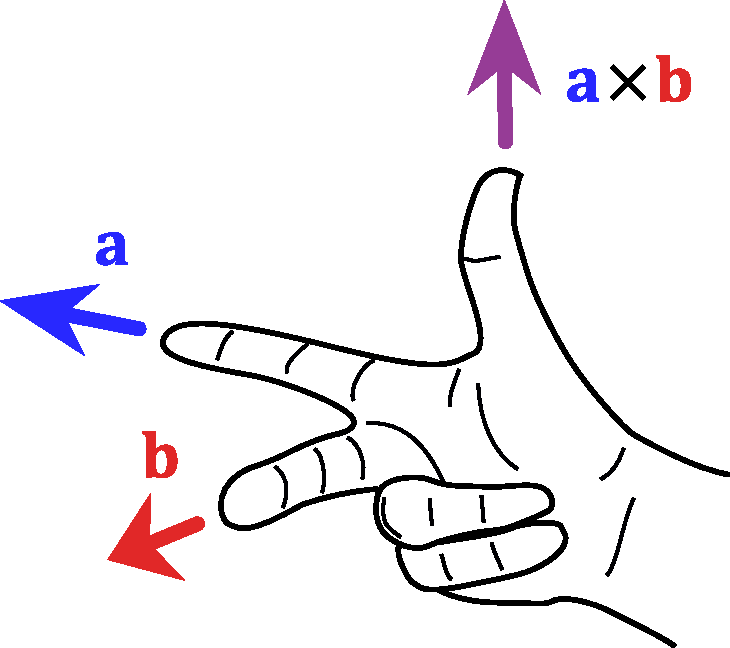
\includegraphics[width=0.3\textwidth]{chapters/vectors/images/right_hand_rule.pdf}
\end{wrapfigure}
\subparagraph{Right-hand rule} The right-hand rule is a simple way to imagine the direction of the vector resulting off a cross product, indeed it is not easy to find it through the Magnitude-Angle notation, nor it is so through Component notation (even though by crunching the numbers it is possible to do so). If done well it is possible to visualize how impossible it is to process the same result by switching the arguments: spoiler it would be of the opposite direction.
    \newpage
    %... so on for all the other chapters
    \documentclass{scrartcl}

\usepackage{amsthm}
\usepackage{amsmath}
\usepackage{amssymb}
\usepackage{siunitx}

\begin{document}
    \section{Motion in Two and Three Dimensions}
    \paragraph{Position Vector} It is a vector that extends from a reference point to a particle. In unit vector notation:
    \begin{equation}
        \vec{r} = x\hat{i}+y\hat{j}+z\hat{k}
    \end{equation}
    \paragraph{Displacement} As the particle moves, the position vector changes. The particle's displacement $\vec{\Delta{r}}$ is:
    \begin{equation}
        \Delta\vec{r}= \vec{r_2} - \vec{r_1}
    \end{equation}
    Or, in unit vector notation:
    \begin{equation}
        \vec{\Delta{r}} = (x_2 - x_1) \hat{i} + (y_2 - y_1) \hat{j} + (z_2 - z_1) \hat{k}
    \end{equation}
    \paragraph{Average Velocity} When a particle moves through a displacement-$\Delta r$ in a time interval $\Delta t$, its average velocity is: 
    \begin{equation}
        \vec{v}_{\mathrm{avg}} = \frac{\Delta\vec{r}}{\Delta t}
    \end{equation}
    The equation clarify that the direction of the velocity is the same as the direction of the displacement.
    In vector notion:
    \begin{equation}
        \vec{v}_{\mathrm{avg}} = \frac{\Delta x \hat{i} + \Delta y \hat{j} + \Delta z \hat{k}}{\Delta t} = \frac{\Delta x}{\Delta t} \hat{i} + \frac{\Delta y}{\Delta t} \hat{j} + \frac{\Delta z}{\Delta t} \hat{k}
    \end{equation}
    \paragraph{Instantaneous Velocity} To find the velocity of a particle at instant \textbf{t} we take the value that $\vec{v}_{\mathrm{avg}}$ assumes as the interval $\Delta t$ approaches to $0$.
    \begin{equation}
        \vec{x} = \frac{d\vec{r}}{dt}
    \end{equation}
    Or, in unit vector notation:
    \begin{equation}
        \vec{v} = v_x \hat{i} + v_y \hat{j} + v_z \hat{k}
    \end{equation}
    Where the scalar components are
    \begin{equation} 
        v_x= \frac{dx}{dt},\quad v_y= \frac{dy}{dt},\quad v_z= \frac{dz}{dt}
    \end{equation}
    \paragraph{Average acceleration} When a particle's velocity changes, its average acceleration $\vec{a}_{avg}$ is
    \begin{equation}
        \vec{a}_{\mathrm{avg}} = \frac{\vec{v}_2 - \vec{v}_1}{\Delta t} = \frac{\Delta \vec{v} }{\Delta t}
    \end{equation}
    \paragraph{Instantaneous Acceleration} As for the velocity, to know the acceleration in an instant $t$, we take the value of $\vec{a}_{\mathrm{avg}}$ assumes as the interval $\Delta{t}$ approaches $0$.
    \begin{equation}
        \vec{a} = \frac{d\vec{v}}{dt}
    \end{equation}
    In unit vector notation:
    \begin{equation}
        \vec{a} = a_x \hat{i} + a_y \hat{j} + a_z \hat{k}
    \end{equation}
    Where the components of $\vec{a}$ are:
    \begin{equation}
        a_x = \frac{dv_x}{dt},\quad a_y = \frac{dv_y}{dt},\quad a_z = \frac{dv_z}{dt}
    \end{equation}
    The direction of an acceleration vectors does not extend from one position to another, it just shows the direction for a particle located at its tail. 
    \paragraph{Projectile motion} A special case of two-dimensional motion, the particle moves with a constant acceleration directed downwards, the free fall acceleration $\vec{g}$. When the projectile is launched, its initial velocity $\vec{v}_0$ is writable as: 
    \begin{equation}
        \vec{v_0} = v_{0x} \hat{i} + v_{0y} \hat{j}
    \end{equation}
    The two components $v_{0x}$ and $v_{0y}$ can be found if we know the angle $\theta_0$ between $\vec{v_0}$ and the positive x direction:
    \begin{equation}
        v_{0x} = v_0 \cos \theta_0,\quad v_{0y} = v_0\sin\theta_0
    \end{equation}
    During the motion both position vector $\vec{r}$ and velocity vector $\vec{v}$ change continuously, though the acceleration remain constant. (There's no horizontal acceleration!)
    The two motions are independent of each other. The horizontal motion has no effect on the vertical one.
    
    \subparagraph{Horizontal motion} Since there is no acceleration, the horizontal component $v_x$ remains unchanged: therefore at any time $t$ the horizontal displacement $x - x_0$ is:
    \begin{equation}
        x - x_0 = v_{0x}t
    \end{equation}
    Since $v_{0x} = v_0 \cos \theta_0$ : 
    \begin{equation}
        x - x_0 = (v_0 \cos \theta_0)t
    \end{equation}
    
    \subparagraph{Vertical motion} Since the acceleration is constant we can apply the equation we have seen in the one dimensional motion chapter. Thus, we have the displacement $y- y_0$
    \begin{equation}
        y - y_0 = (v_{0} \sin \theta_0)t - \frac{1}{2}gt^2
    \end{equation}
    
    Similarly, for the final velocity $v_y$
    \begin{equation}
        v_y = v_0 \sin \theta_0 - gt 
    \end{equation}
    and
    \begin{equation}
        v^2_y = (v_0 \sin \theta_0)^2 - 2g(y-y_0)
    \end{equation}
    \subparagraph{The Equation of the path} We can find the equation of the path of the projectile (called \emph{trajectory}) by solving equation (16) for $t$ and substituting into equation (17).
    \begin{equation}
        y = (\tan \theta_0)x - \frac{gx^2}{2(v_0 \cos \theta_0)^2}
    \end{equation}
    \subparagraph{The Horizontal Range} The horizontal distance the projectile has traveled when it returns to its initial height is called Horizontal Range $R$:
    \begin{equation}
        R = \frac{v^2_0}{g} \sin \theta_0 \cos \theta_0
    \end{equation}
    The maximum horizontal range $R$ is maximum at angle $\theta = 45^o$.
    
    Calculation done with the formula seen in this paragraph may differ a lot with the actual motion of the projectile as we assume the air has no effect on the projectile. 
    
    \paragraph{Uniform Circular Motion} A particle in uniform circular motion travels around a circle or a circular arc at constant speed. However, since the particle is moving in circles the direction of the velocity changes, thus the particle is accelerating. Velocity is always directed tangent to the circle in the direction of motion, while the acceleration is directed radially inward. Because of this, the acceleration is called centripetal acceleration. The magnitude of this acceleration $\vec{a}$ is:
    \begin{equation}
        a = \frac{v^2}{r}
    \end{equation}
    where r is the radius of the circle and v is the speed.
    
    During the motion, the particle travels the circumference of the circle in time $T$:
    \begin{equation}
        T = \frac{2\pi r}{v}
    \end{equation}
    $T$ is called \emph{period of revolution} or simply \emph{period}.
    
    \paragraph{Relative Motion in One Dimension} The velocity of a particle depends on the reference frame of whoever is observing it. Let's have two reference frames A and B, both observing a particle P, then the following equations hold:
    \begin{itemize}
        \item Position:
        \begin{equation}
            x_{\mathrm{PA}} = x_{\mathrm{PB}} + x_{\mathrm{BA}}
        \end{equation}
        To obtain the velocity equation we take the time derivative of equation (24)
        \item Velocity:
        \begin{equation}
            v_{\mathrm{PA}} = v_{\mathrm{PB}} + v_{\mathrm{BA}}
        \end{equation}
        To obtain the acceleration equation we take the time derivative of equation (25), since $v_{\mathrm{BA}}$ is constant the derivative will be $0$.
        \item Acceleration:
        \begin{equation}
            a_{\mathrm{PA}} = a_{\mathrm{PB}}
        \end{equation}
        Observers on different frames of reference that move at constant velocity relative to each other will measure the same acceleration for a moving particle.
    \end{itemize}
    \paragraph{Relative Motion in Two Dimensions} Similarly in two dimensions, having two reference frames A and B, both observing a particle P, the following equation holds:
    \begin{itemize}
        \item Position Vector:
        \begin{equation}
            \vec{r}_{\mathrm{PA}} = \vec{r}_{\mathrm{PB}} + \vec{r}_{\mathrm{BA}}
        \end{equation}
        To obtain the velocity equation we take the time derivative of equation (27)
        \item Velocity:
        \begin{equation}
            \vec{v}_{\mathrm{PA}} = \vec{v}_{\mathrm{PB}} + \vec{v}_{\mathrm{BA}}
        \end{equation}
        To obtain the acceleration equation we take the time derivative of equation (25), since $v_{\mathrm{BA}}$ is constant the derivative will be $0$.
        \item Acceleration:
        \begin{equation}
            a_{\mathrm{PA}} = a_{\mathrm{PB}}
        \end{equation}
        The same rule of One Dimensional motion holds, observers on different frames of reference that move at constant velocity relative to each other will measure the same acceleration for a moving particle. 
    \end{itemize}
\end{document}
\end{document}
